\documentclass[aspectratio=169,11pt]{beamer}

\usetheme{metropolis}
\usecolortheme{default}
\setbeamertemplate{navigation symbols}{}
\setbeamertemplate{footline}{%
  \hfill\usebeamerfont{page number in head/foot}\insertframenumber\hspace{3mm}\vspace{2mm}
}

\usepackage[T1]{fontenc}
\usepackage[utf8]{inputenc}
\usepackage{booktabs}
\usepackage{tikz}
\usepackage{pgfplots}
\usepackage{amsmath}
\usepackage{array}
\usepackage{xcolor}
\usepackage{appendixnumberbeamer}

\usetikzlibrary{arrows.meta,positioning,calc,fit,shapes.geometric,decorations.pathreplacing}
\pgfplotsset{compat=1.18}

\definecolor{sbbred}{HTML}{E0001B}
\definecolor{ink}{HTML}{202124}
\definecolor{muted}{HTML}{5F6368}
\definecolor{track}{HTML}{2E5EAA}
\definecolor{walk}{HTML}{D9822B}
\definecolor{okgreen}{HTML}{16803C}
\definecolor{warn}{HTML}{B45309}
\definecolor{softblue}{HTML}{EAF2FF}
\definecolor{softgreen}{HTML}{EAF7EF}
\definecolor{softorange}{HTML}{FFF2E0}
\definecolor{softred}{HTML}{FDE8EA}

\setbeamercolor{normal text}{fg=ink,bg=white}
\setbeamercolor{frametitle}{fg=ink,bg=white}
\setbeamercolor{progress bar}{fg=sbbred,bg=softred}
\setbeamercolor{alerted text}{fg=sbbred}

\newcommand{\ph}[1]{\textcolor{warn}{\textbf{PLACEHOLDER: #1}}}
\newcommand{\smallcap}[1]{\textcolor{muted}{\scriptsize\MakeUppercase{#1}}}
\newcommand{\metric}[2]{%
  \begin{tabular}{@{}c@{}}
    {\Large\bfseries #1}\\[-1mm]
    {\scriptsize\textcolor{muted}{#2}}
  \end{tabular}}

\title{Robust Journey Planning for SBB}
\subtitle{Fastest route that still arrives on time with probability at least $Q$}
\author{Zhixiang Dai, Weijiang Xiong, Jinghao Zheng, Kaile Chu}
% \author{Z. Dai, W. Xiong, J. Zheng, K. Chu}
\date{May 27, 2026}

\begin{document}

% ---------------------------------------------------------------------------
\begin{frame}
  \titlepage
  \vspace{-6mm}
  \begin{center}
    \smallcap{7-minute video storyline: methodology, viability, validation}
  \end{center}
\end{frame}

% ---------------------------------------------------------------------------
\begin{frame}{The Question We Answer}

  \vspace{-3mm}
  \begin{columns}[T,onlytextwidth]
    \column{0.49\textwidth}
      \begin{block}{Input}
        \begin{itemize}
          \item origin stop $A$, destination stop $B$
          \item weekday and latest arrival time $T$
          \item confidence threshold $Q$
          \item region UUID list from \texttt{geo}
        \end{itemize}
      \end{block}

    \vspace{-2.5mm}  
      \begin{block}{Output}
      \begin{itemize}
          \item Routes arriving before $T$ with confidence $\ge Q$, sorted by latest departure time.
      \end{itemize}
      \end{block}

    \column{0.49\textwidth}
      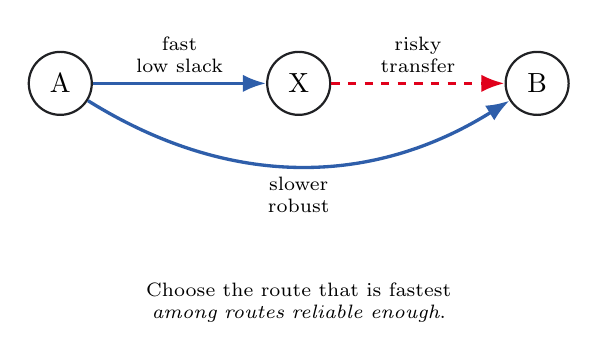
\begin{tikzpicture}[node distance=8mm,>=Latex,
          stop/.style={circle,draw=ink,fill=white,minimum size=8mm,thick},
          route/.style={draw=track,very thick,-Latex},
          risky/.style={draw=sbbred,very thick,-Latex,dashed},
          lab/.style={font=\scriptsize,align=center}]
        \node[stop] (A) {A};
        \node[stop,right=22mm of A] (X) {X};
        \node[stop,right=22mm of X] (B) {B};
        \draw[route] (A) -- node[lab,above]{fast\\low slack} (X);
        \draw[risky] (X) -- node[lab,above]{risky\\transfer} (B);
        \draw[route,bend right=32] (A) to node[lab,below]{slower\\robust} (B);
        \node[lab,below=20mm of X,text width=65mm] {
          Choose the route that is fastest \emph{among routes reliable enough}.
        };
      \end{tikzpicture}
  \end{columns}

  \begin{alertblock}{Main assumptions}
    \vspace{1mm}
    Latest timetable week; no holiday exceptions; walking is deterministic at 50 m/min; route leg delays are combined under an independence assumption.
  \end{alertblock}
\end{frame}

% ---------------------------------------------------------------------------
\begin{frame}{System Overview}
  \centering

    \resizebox{\textwidth}{!}{\input{fig_system_overview.tex}}

  \vspace{2mm}
  \only<1>{\smallcap{Build a planner from timetable, history, and geography.}}
  \only<2>{\smallcap{Preparation builds reusable regional tables and delay distributions.}}
  \only<3>{\smallcap{Each user query runs routing plus confidence scoring.}}
\end{frame}

% ---------------------------------------------------------------------------
\begin{frame}{Data Structure: A Time-Dependent Transit Graph}
  \begin{columns}[T,onlytextwidth]
    \column{0.54\textwidth}
    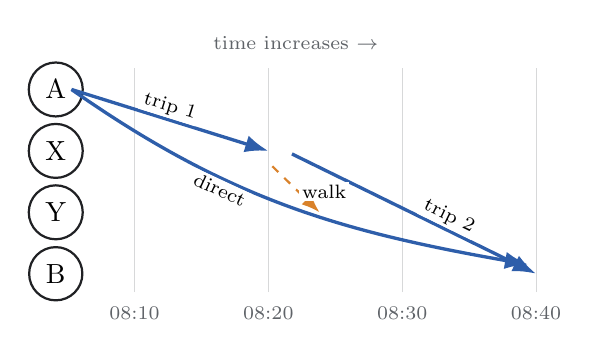
\begin{tikzpicture}[x=1cm,y=0.78cm,>=Latex,
        stop/.style={circle,draw=ink,fill=white,minimum size=6mm,thick},
        ride/.style={draw=track,very thick,-Latex},
        walkedge/.style={draw=walk,thick,dashed,-Latex},
        time/.style={font=\scriptsize,text=muted},
        edgelabel/.style={font=\scriptsize,fill=white,inner sep=1pt}]
      \foreach \y/\name in {3/A,2/X,1/Y,0/B}{
        \node[stop] (\name) at (0,\y) {\name};
      }
      \foreach \x/\t in {1/08:10,2.7/08:20,4.4/08:30,6.1/08:40}{
        \node[time] at (\x,-0.65) {\t};
        \draw[muted!25] (\x,-0.3) -- (\x,3.35);
      }
      \draw[ride] (0.2,3) -- node[edgelabel,above,sloped,pos=0.48]{trip 1} (2.7,2);
      \draw[ride] (3.0,1.95) -- node[edgelabel,above,sloped,pos=0.62]{trip 2} (6.1,0);
      \draw[ride] (0.2,3) to[out=-35,in=170]
        node[edgelabel,below,sloped,pos=0.35]{direct} (6.0,0.15);
      \draw[walkedge] (2.75,1.75) -- node[edgelabel,right,pos=0.55]{walk} (3.35,1.0);
      \node[time] at (3.05,3.75) {time increases $\rightarrow$};
    \end{tikzpicture}

    \column{0.42\textwidth}
    \begin{itemize}
      \item Stops are normalized to station-level IDs.
      \item Trips become ordered stop-time sequences.
      \item Walking edges are generated within the configured radius.
      \item Service availability is filtered by weekday calendar flags.
    \end{itemize}

    \vspace{2mm}
    \begin{block}{Implementation detail}
      \texttt{prepare(regions=[...])} rebuilds regional \texttt{stops}, \texttt{stop\_to\_stop}, and \texttt{stop\_times}.
    \end{block}
  \end{columns}
\end{frame}

% ---------------------------------------------------------------------------
\begin{frame}{Delay Model: Probability From Historical Slack}
  \begin{columns}[T,onlytextwidth]
    \column{0.48\textwidth}
      \begin{block}{Training signal}
        \small
        \[
          \mathrm{delay}
          = t_{\mathrm{actual\ arrival}}
          - t_{\mathrm{scheduled\ arrival}}
        \]
      \end{block}

      Clean Istdaten records:
      \begin{itemize}
        \item planned and actual arrival known
        \item not failed, not unplanned
        \item arrival status marked as real
      \end{itemize}

      \vspace{1mm}
      Profiles are grouped by:
      \[
        \text{stop} \times \text{weekday} \times \text{hour}
      \]

    \column{0.48\textwidth}
      \centering
      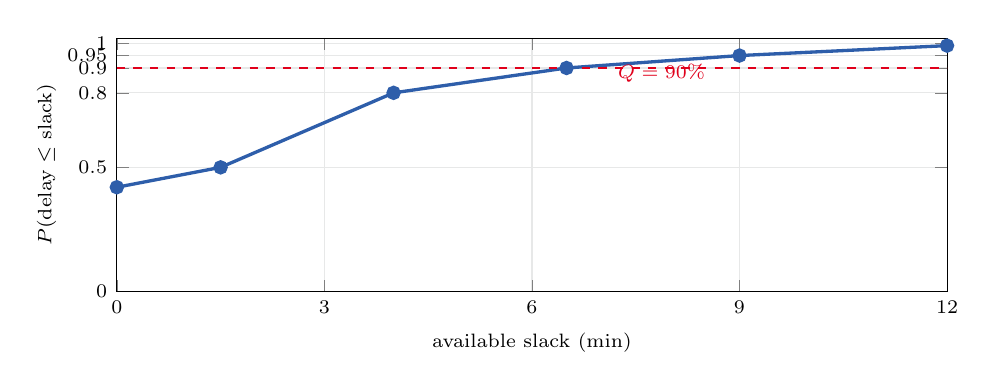
\begin{tikzpicture}
        \begin{axis}[
          width=\linewidth,height=48mm,
          xmin=0,xmax=12,ymin=0,ymax=1.02,
          xlabel={available slack (min)},
          ylabel={$P(\mathrm{delay}\le\mathrm{slack})$},
          ylabel style={yshift=-1mm},
          grid=both,
          grid style={draw=muted!15},
          tick label style={font=\scriptsize},
          label style={font=\scriptsize},
          ytick={0,0.5,0.8,0.9,0.95,1},
          xtick={0,3,6,9,12}]
          \addplot[track,very thick,mark=*] coordinates {(0,0.42) (1.5,0.50) (4,0.80) (6.5,0.90) (9,0.95) (12,0.99)};
          \addplot[sbbred,dashed,thick] coordinates {(0,0.9) (12,0.9)};
          \node[font=\scriptsize,anchor=west,text=sbbred] at (axis cs:7.1,0.88) {$Q=90\%$};
        \end{axis}
      \end{tikzpicture}

      \vspace{-1mm}
      {\scriptsize\textcolor{muted}{QUANTILE PROFILES SCORE ANY SLACK VALUE.}}
  \end{columns}
\end{frame}

% ---------------------------------------------------------------------------
\begin{frame}{How Confidence Enters a Route}
  \centering
  \begin{tikzpicture}[>=Latex,
      stop/.style={circle,draw=ink,fill=white,minimum size=8mm,thick},
      ride/.style={draw=track,very thick,-Latex},
      walkedge/.style={draw=walk,thick,dashed,-Latex},
      prob/.style={font=\scriptsize,align=center,fill=white}]
    \node[stop] (A) at (0,0) {A};
    \node[stop] (X) at (2.7,0) {X};
    \node[stop] (Y) at (5.2,0) {Y};
    \node[stop] (B) at (7.9,0) {B};

    \draw[ride] (A) -- node[prob,above=2mm] {$p_1=P(d_X \le s_X)$} (X);
    \draw[walkedge] (X) -- node[prob,below=2mm] {deterministic walk\\debits slack} (Y);
    \draw[ride] (Y) -- node[prob,above=2mm] {$p_2=P(d_B \le T-t_B)$} (B);

    \only<2->{
      \node[draw=okgreen,fill=softgreen,rounded corners=1mm,align=center,text width=80mm,below=13mm of Y] {
        \small Route confidence:
        $P(\mathrm{route\ succeeds}) \approx \prod_{\mathrm{ride\ legs}} p_i$
      };
    }
    \only<3->{
      \node[draw=sbbred,fill=softred,rounded corners=1mm,align=center,text width=82mm,above=11mm of Y] {
        \small Keep only if confidence $\ge Q$ and arrival $\le T$.
      };
    }
  \end{tikzpicture}

  \vspace{1mm}
  \only<1>{\smallcap{Each transfer/final deadline creates a slack value.}}
  \only<2>{\smallcap{The project allows assuming independent delay events.}}
  \only<3>{\smallcap{Reliability filters routes before ranking.}}
\end{frame}

% ---------------------------------------------------------------------------
\begin{frame}{Routing Algorithm}
  \begin{columns}[T,onlytextwidth]
    \column{0.50\textwidth}
      \begin{block}{Candidate generation}
        \begin{enumerate}
          \item Sweep departure probes backward from $T$.
          \item Run Multi-Criteria RAPTOR for each probe.
          \item Keep Pareto journeys by arrival time, walking distance, and transfers.
          \item Score each route with the empirical confidence model.
        \end{enumerate}
      \end{block}

      \vspace{1mm}
      \begin{alertblock}{Ranking contract}
        Return routes with confidence $\ge Q$, sorted from latest departure to earliest departure.
      \end{alertblock}

    \column{0.46\textwidth}
      \begin{tikzpicture}[>=Latex,node distance=8mm,
          box/.style={draw=ink,rounded corners=1mm,align=center,minimum width=39mm,minimum height=8mm,fill=white,font=\scriptsize},
          arr/.style={-Latex,very thick,draw=muted}]
        \node[box,fill=softblue] (q) {query $(A,B,T,Q,\mathrm{day})$};
        \node[box,fill=softorange,below=of q] (sweep) {departure sweep\\$T,T-5,\dots,T-W$};
        \node[box,fill=softgreen,below=of sweep] (rap) {McRAPTOR\\Pareto labels};
        \node[box,fill=softred,below=of rap] (score) {confidence scoring\\filter $\ge Q$};
        \node[box,fill=white,below=of score] (rank) {deduplicate and sort};
        \draw[arr] (q) -- (sweep);
        \draw[arr] (sweep) -- (rap);
        \draw[arr] (rap) -- (score);
        \draw[arr] (score) -- (rank);

        \only<2->{\node[draw=sbbred,rounded corners=1mm,fit=(sweep),inner sep=1.5mm] {};}
        \only<3->{\node[draw=okgreen,rounded corners=1mm,fit=(rap),inner sep=1.5mm] {};}
      \end{tikzpicture}
  \end{columns}
\end{frame}

% ---------------------------------------------------------------------------
\begin{frame}{Validation: Does the Probability Mean What It Says?}
  \begin{columns}[T,onlytextwidth]
    \column{0.46\textwidth}
      \begin{block}{Strict time split}
        \begin{itemize}
          \item Training: max date $-365$ days to max date $-30$ days
          \item Test: final 30 days, never used in training
          \item No future information is used
        \end{itemize}
      \end{block}

      \begin{block}{Metrics}
        \small
        \begin{itemize}
          \item calibration error at p50, p80, p90, p95
          \item per-stop calibration error
          \item robust planner vs. fastest-route baseline
        \end{itemize}
      \end{block}

    \column{0.50\textwidth}
      \centering
      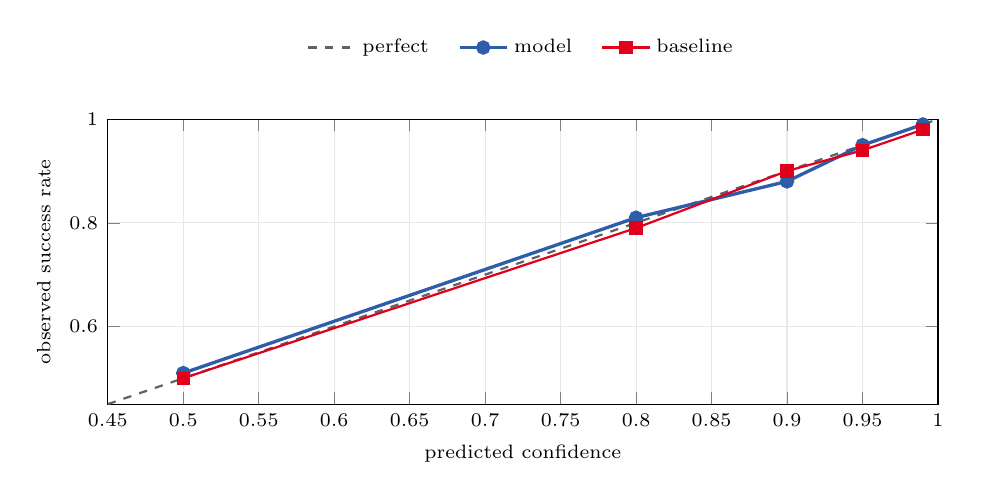
\begin{tikzpicture}
        \begin{axis}[
          width=\linewidth,height=52mm,
          xmin=0.45,xmax=1.0,ymin=0.45,ymax=1.0,
          xlabel={predicted confidence},
          ylabel={observed success rate},
          grid=both,
          grid style={draw=muted!15},
          tick label style={font=\scriptsize},
          label style={font=\scriptsize},
          legend style={
            font=\scriptsize,
            at={(0.5,1.18)},
            anchor=south,
            legend columns=3,
            draw=none,
            fill=none,
            /tikz/every even column/.append style={column sep=3mm}
          }]
          \addplot[muted,dashed,thick] coordinates {(0.45,0.45) (1,1)};
          \addlegendentry{perfect}
          \addplot[track,very thick,mark=*] coordinates {(0.50,0.51) (0.80,0.81) (0.90,0.88) (0.95,0.95) (0.99,0.99)};
          \addlegendentry{model}
          \addplot[sbbred,thick,mark=square*] coordinates {(0.50,0.50) (0.80,0.79) (0.90,0.90) (0.95,0.94) (0.99,0.98)};
          \addlegendentry{baseline}
        \end{axis}
      \end{tikzpicture}

      \vspace{-2mm}
      \ph{Insert final calibration values from cluster run.}
  \end{columns}
\end{frame}

% ---------------------------------------------------------------------------
\begin{frame}{Validation Finding: Morning Peak Risk}
  \begin{columns}[T,onlytextwidth]
    \column{0.53\textwidth}
      \centering
      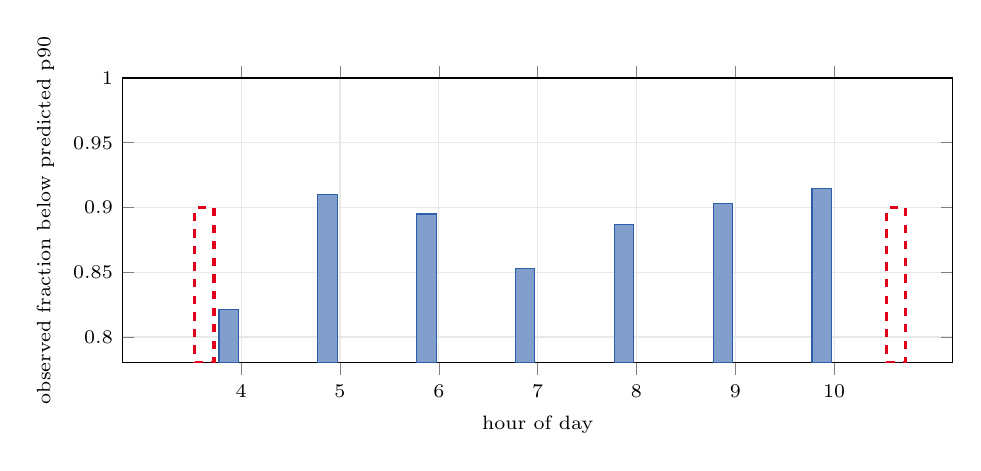
\begin{tikzpicture}
        \begin{axis}[
          ybar,
          width=\linewidth,height=52mm,
          ymin=0.78,ymax=1.0,
          xlabel={hour of day},
          ylabel={observed fraction below predicted p90},
          xtick={4,5,6,7,8,9,10},
          ytick={0.8,0.85,0.9,0.95,1.0},
          grid=major,
          grid style={draw=muted!15},
          tick label style={font=\scriptsize},
          label style={font=\scriptsize},
          bar width=7pt]
          \addplot[fill=track!60,draw=track] coordinates {(4,0.821) (5,0.91) (6,0.895) (7,0.853) (8,0.887) (9,0.903) (10,0.915)};
          \addplot[sbbred,dashed,very thick] coordinates {(3.5,0.9) (10.5,0.9)};
        \end{axis}
      \end{tikzpicture}

      \ph{Replace with final hourly p90 chart if rerun.}

    \column{0.43\textwidth}
      \begin{block}{Interpretation}
        The empirical model is broadly calibrated, but morning-peak cascade delays are harder to capture.
      \end{block}

      \begin{itemize}
        \item Hour 7 is the known weak point in the current notebook.
        \item This is statistically meaningful when the test count is large.
        \item For 07:00 journeys, the planner may over-promise unless extra buffer is required.
      \end{itemize}

      \vspace{1mm}
      \smallcap{This limitation is part of the method, not hidden from the user.}
  \end{columns}
\end{frame}

% ---------------------------------------------------------------------------
\begin{frame}{Operational Example}
  \begin{columns}[T,onlytextwidth]
    \column{0.45\textwidth}
      \begin{block}{Query}
        \begin{tabular}{@{}ll@{}}
          Origin & EPFL \textcolor{warn}{(TBD stop ID)}\\
          Destination & CHUV \textcolor{warn}{(TBD stop ID)}\\
          Day & \textcolor{warn}{TBD}\\
          Arrival deadline & 09:00\\
          Confidence & 90\%\\
          Walking budget & 500 m
        \end{tabular}
      \end{block}

      \begin{block}{Result to show}
        \begin{tabular}{@{}lll@{}}
          \toprule
          dep. & arr. & confidence\\
          \midrule
          \textcolor{warn}{08:xx} & \textcolor{warn}{08:xx} & \textcolor{warn}{9x\%}\\
          \textcolor{warn}{08:xx} & \textcolor{warn}{08:xx} & \textcolor{warn}{9x\%}\\
          \bottomrule
        \end{tabular}
      \end{block}

    \column{0.51\textwidth}
      \centering
      \resizebox{\linewidth}{!}{%
      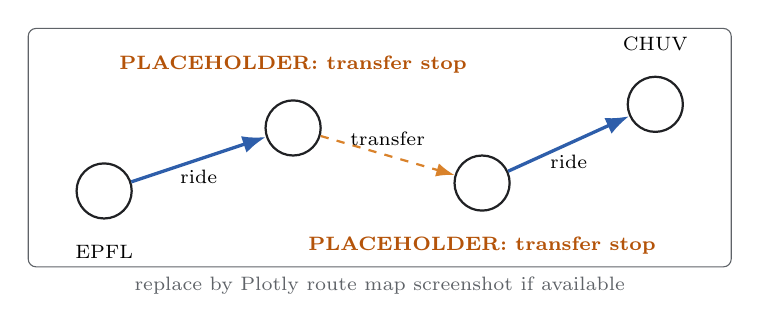
\begin{tikzpicture}[>=Latex,
          stop/.style={circle,draw=ink,fill=white,minimum size=7mm,thick},
          ride/.style={draw=track,very thick,-Latex},
          walkedge/.style={draw=walk,thick,dashed,-Latex},
          lab/.style={font=\scriptsize,align=center}]
        \node[stop] (epfl) at (0,0) {};
        \node[stop] (renens) at (2.4,0.8) {};
        \node[stop] (laus) at (4.8,0.1) {};
        \node[stop] (chuv) at (7.0,1.1) {};
        \draw[ride] (epfl) -- node[lab,below]{ride} (renens);
        \draw[walkedge] (renens) -- node[lab,above]{transfer} (laus);
        \draw[ride] (laus) -- node[lab,below]{ride} (chuv);
        \node[lab,below=2mm of epfl] {EPFL};
        \node[lab,above=2mm of renens] {\ph{transfer stop}};
        \node[lab,below=2mm of laus] {\ph{transfer stop}};
        \node[lab,above=2mm of chuv] {CHUV};
        \node[draw=muted,rounded corners=1mm,fit=(epfl)(renens)(laus)(chuv),inner sep=6mm,label={[font=\scriptsize,text=muted]below:replace by Plotly route map screenshot if available}] {};
      \end{tikzpicture}
      }

      \vspace{2mm}
      \smallcap{Optional demo: 15--20 seconds of notebook widget or Plotly map.}
  \end{columns}
\end{frame}

% ---------------------------------------------------------------------------
\begin{frame}{What We Can Claim}
  \small
  \begin{columns}[T,onlytextwidth]
    \column{0.50\textwidth}
      \begin{block}{Strengths}
        \begin{itemize}
          \item Region-agnostic initialization via geo UUIDs.
          \item Explainable delay model tied directly to route slack.
          \item Standard public-transit algorithm adapted to walking and reliability constraints.
          \item Validation uses held-out future days, avoiding leakage.
        \end{itemize}
      \end{block}

    \column{0.46\textwidth}
      \begin{alertblock}{Limitations}
        \begin{itemize}
          \item Independence assumption between leg delays.
          \item Walking is straight-line and deterministic.
          \item McRAPTOR candidates are Pareto by arrival/walking/transfers before confidence scoring.
          \item Morning-peak reliability is currently less well calibrated.
        \end{itemize}
      \end{alertblock}
  \end{columns}

  \vspace{2mm}
  \begin{center}
    \normalsize\bfseries
    The planner returns the fastest route that is reliable enough.
  \end{center}
\end{frame}

% ---------------------------------------------------------------------------
\appendix
\begin{frame}{Backup: Suggested Final Numbers To Fill In}
  \begin{itemize}
    \item Region names and UUIDs used in the video.
    \item Counts after preprocessing: stops, walking edges, stop-time rows, grouped routes.
    \item Delay-profile rows and training/test date range.
    \item Calibration table: target quantile, observed fraction, Wilson CI, error.
    \item Per-stop calibration error vs. global baseline.
    \item One route example: departure, arrival, confidence, transfer slack.
    \item Runtime: preparation time and one-query routing time.
  \end{itemize}
\end{frame}

\end{document}
